\documentclass{article}
\usepackage{graphicx} % Required for inserting images
\usepackage{amsmath}
\usepackage{amsfonts}
\usepackage{cleveref}

\title{Intepretation of the Wasserstein Impact Measure}
\author{Damian Mingo, Jack S. Hale}
\date{June 2023}

\begin{document}


\maketitle

\section{Introduction}
Several measures of prior impact assessment have been developed. These measures of prior impact are usually based on divergences such as the Kullback–Leibler divergence or distances such as the Wasserstein distance. However, these distances are not directly interpretable and cannot tell us the weight of the impact of a prior distribution. We provide the weight of impact for prior distributions relative to standard normal distributions.

\section{Methodology}
\subsection{Calculation of the Wasserstein distance}

\subsection{Normalisation with prior distances}

\subsection{Power posteriors}

\section{Examples}

\subsection{Normal-normal conjugate case with unknown mean}
Following standard arguments, it is possible to show that the distribution of
the power posterior for the following Bayesian model with dataset $x = (x_1,
\ldots, x_n)$
\begin{subequations}
\begin{align}
	x_1, \ldots, x_n &\overset{\mathrm{iid}}{\sim} \mathcal{N}(m, \sigma^2), \\
m &\sim \mathcal{N}(m_0, \sigma_0^2),
\end{align}
\end{subequations}
is normally distributed
\begin{equation*}
m \;|\; x \sim \mathcal{N} \left( \left( \frac{1}{\sigma_0^2} + \frac{\gamma n}{\sigma^2} \right)^{-1} \left(\frac{m_0}{\sigma_0^2} + \frac{\gamma n \bar{x}}{\sigma^2}  \right), \left( \frac{1}{\sigma_0^2} + \frac{\gamma n}{\sigma^2} \right)^{-1} \right),
\end{equation*}
where $\bar{x} = (\sum x_i)/ n$ is the sample mean. We remark that, as
expected, the prior is recovered when $\gamma = 0$ and the classic
normal-normal with unknown mean conjugate result is recovered when $\gamma =
1$. The role of $\gamma$ in this context is to reduce the contribution of each
element of the dataset through the likelihood. More specifically for the
normal-normal case, the effective data set size is reduced from the standard
posterior ($\gamma = 1$) from $n$ to $n \gamma$ in the power posterior. Note
however, regardless of the value of $\gamma > 0$, the entire dataset $x$ is
still used in the update from prior to the power posterior.

The 2-Wasserstein metric ($p = 2$) for two non-degenerate normal
measures $\mu_1$ and $\mu_2$ on $\mathbb{R}$ with means $m_1, m_2 \in
\mathbb{R}$ and variances $\sigma_1^2, \sigma_2^2 \in \mathbb{R}_{>0} :=
\left\lbrace x \in \mathbb{R} \; | \; x > 0 \right\rbrace$, respectively, can
be found in closed form as
\begin{equation*}
W_{2} (\mu_1, \mu_2)^2 = \left( m_1 - m_2 \right)^2 + \sigma_1^2 + \sigma_2^2 - 2 \bigl( \sigma_2 \sigma_1^2 \sigma_2 \bigr)^{1/2}.
\end{equation*}
Consequently in this case there is no need to resort to approximate numerical
computations to compute the Wasserstein metric. In closed form the Wasserstein
metric between the prior measure $\mu_0$ and the measure induced by the power posterior
$\mu_\gamma$ is
\begin{equation*}
W_2(\mu_0, \mu_\gamma)^2 = \sigma_{0}^{2} + \frac{\sigma^{2} \sigma_{0}^{2}}{p} + \frac{\left(\gamma m_{0} n \sigma_{0}^{2} - \gamma n \sigma_{0}^{2} \bar{x}\right)^{2}}{p^{2}} - \frac{2 \sigma \sigma_{0}^{2}}{\sqrt{p}}
\end{equation*}
with $p = \gamma n \sigma_{0}^{2} + \sigma^{2}$ and the derivative of the
squared Wasserstein distance with respect to $\gamma$ given by
\tiny
\begin{equation*}
\frac{d}{d\gamma} [W_2(\mu_0, \mu_\gamma)^2] =
p^{-\frac{15}{2}}n \sigma_{0}^{2} \left(- p^{\frac{11}{2}} \sigma^{2} \sigma_{0}^{2} - 2 p^{\frac{9}{2}} \left(- \gamma n \sigma_{0}^{2} \bar{x} + m_{0} p - m_{0} \sigma^{2}\right) \left(- \gamma n \sigma_{0}^{2} \bar{x} - m_{0} \sigma^{2} + p \bar{x}\right) + p^{6} \sigma \sigma_{0}^{2}\right).
\end{equation*}
\normalsize
Letting $\gamma = 0$ it can be verified that $W_2(\mu_0, \mu_0)^2 = 0$, as
expected, and also that $\frac{d}{d\gamma}[W_2(\mu_0, \mu_0)^2] = 0$. 

In the first experiment we generate a (small) dataset of size $n = 10$ from a
normal distribution with zero mean and unit variance. We propose three prior
choices by adjusting the prior parameters $m_0$ and $\sigma_0^2$:
\begin{enumerate}
\item \emph{Non-informative prior}. $m_0 = 0$ and $\sigma_0^2 = 100$. With
this relatively flat prior we expect the posterior to be `data prominent'
and highly sensitive to the inclusion of information via the likelihood,
here controlled by the parameter $\gamma$.
\item \emph{Informative `correct' prior}. $m_0 = 0$ and $\sigma_0^2 = 2$.
This prior expresses definite information about the parameter that
coincidentally coincides with the true parameter. 
\item \emph{Informative `incorrect' prior}. $m_0 = -5$ and $\sigma_0^2 = 2$.
This prior expresses definite information about the parameter that
does not coincide with the true parameter value. 
\end{enumerate}
In \cref{fig:normal_normal_wasserstein_distance_different_priors} we calculate
the squared 2-Wasserstein distance between the posterior measure $\mu_\gamma$
for varying values of $\gamma$ and under the three prior assumptions just
described. All three distances appear to be monotonically increasing in
$\gamma$. The distance between the posterior and prior as $\gamma \to 1$ is
largest ($\sim10^2$) for the non-informative prior, and smallest ($\sim 1$) for
the informative `correct' prior. For the non-informative prior as $\gamma$ is
increased from $0$ we can see a very sudden increase in the metric, which
supports the intuition that the posterior is `data prominent' or `data
sensitive`. By comparison, the distance for the informative `correct' prior
evolves to its final distance more slowly, reflecting that the information
contained in the prior does not strongly disagree with that in the data. The
informative `incorrect' prior sits in between the two extreme cases.
\begin{figure}
\begin{center}
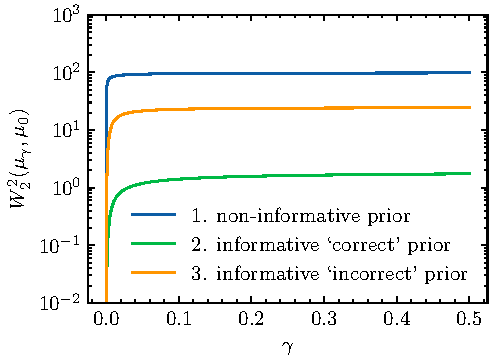
\includegraphics{imgs/normal_normal_wasserstein_distance_different_priors.pdf}
\end{center}
\caption{Normal-normal conjugate case; plot showing squared
2-Wasserstein metric between power posterior and prior against the
power posterior parameter $\gamma \in [0, \frac{1}{2}]$ under the three
different prior assumptions described in the text.}\label{fig:normal_normal_wasserstein_distance_different_priors}
\end{figure}

Given the intepretation of the parameter $\gamma n$ as an effective sample size
in the normal-normal setting, we briefly contrast the power posterior approach
with an approach based on using the standard posterior and varying the size $n$
of the dataset.

\subsection{Inverse-Gamma conjugate case with unknown variance}
Following standard arguments, it is possible to show that the distribution of
the power posterior for the following Bayesian model with dataset $x = (x_1,
\ldots, x_n)$
\begin{subequations}
\begin{align}
x_1, \ldots, x_n &\overset{\mathrm{iid}}{\sim} \mathcal{N}(m, \sigma^2), \\
\sigma^2 &\sim \text{Inv-Gamma}(\alpha, \beta)
\end{align}
\end{subequations}
with $\alpha, \beta \in \mathbb{R}_{>0}$, is distributed according to an
inverse gamma distribution
\begin{equation*}
\sigma^2 \; | \; x_1, \ldots, x_n \sim \text{Inv-Gamma}\left( \alpha + \frac{\gamma n}{2}, \beta + \frac{\gamma n}{2} s^2 \right). 
\end{equation*}
where $s^2 = (\sum_{i} \left( x_i - \mu \right)^2)/n$ is the uncorrected sample
variance. Again, setting $\gamma = 0$ recovers the prior, and setting $\gamma =
1$ recovers the usual conjugate result for the standard Bayesian posterior.

To the best of our knowledge there is no easily computable expression for the
Wasserstein metric between inverse gamma distributions for any value of $p$.
We instead use the Vallender formula which relates the 1-Wasserstein distance
between two probability measures $\mu_1$ and $\mu_2$ on $\mathbb{R}$ with
cumulative distribution functions $F_1(x)$ and $F_2(x)$, respectively
\begin{equation}
W_1(\mu_1, \mu_2) = \int_{\mathbb{R}} | F_1(x) - F_2(x) | \; \mathrm{d}x.
\end{equation}


\subsection{Poisson-Gamma conjugate case with unknown rate}
The distribution of the power posterior of the following Bayesian model with
dataset $x = (x_1, \ldots, x_n)$ 
\begin{subequations}
\begin{align}
x_1, \ldots, x_n &\overset{\mathrm{iid}}{\sim} \text{Poisson}(\lambda), \\
\lambda &\sim \text{Gamma}(\alpha, \beta),
\end{align}
\end{subequations}
where $\lambda \in \mathbb{R}_{>0}$ is the unknown rate parameter, and $\alpha,
\beta \in \mathbb{R}_{>0}$ are prior parameters is given by
\begin{equation}
\lambda \; | \; x \sim \text{Gamma} \left( \alpha + \gamma n \bar{x}, \beta + \gamma n \right)
\end{equation}

\section{Conclusion}

\end{document}
